 
\chapter{Systems of linear equations and inequalities}
\label{chap_systems_lin_eq}
\mfpicnumber{1}
\opengraphsfile{LinSystems}
\graphicspath{{figures/Systems_lin_eq/}}

\setlength{\extrarowheight}{0pt}


\section{Systems of linear equations} \label{syst_lin_eq}

Up until now, when we concerned ourselves with solving different types of equations there was only one equation to solve at a time.  Given an equation $f(x) = g(x)$, we could check our solutions geometrically by finding where the graphs of $y=f(x)$ and $y=g(x)$ intersect. The $x$-coordinates of these intersection points correspond to the solutions to the equation $f(x) = g(x)$, and the $y$-coordinates were largely ignored.  If we modify the problem and ask for the intersection points of the graphs of $y=f(x)$ and $y=g(x)$, where both the solution to $x$ and $y$ are of interest, we have what is known as a \index{system of equations ! definition} \textbf{system of equations} (\textit{stelsel van vergelijkingen}), usually written as
 \[ \left\{ \begin{array}{rcl} y & = & f(x) \\ y & = & g(x). \\ \end{array} \right.\]  
The 'curly bracket' notation means we are  to find all pairs of points $(x,y)$ which satisfy both equations.  We begin our study of systems of equations by reviewing some basic notions from intermediate algebra.

\smallskip


\begin{definition}[Linear equation in two variables]
	\label{lineareqntwovariables}  A \index{equation ! linear of two variables} \index{linear equation ! two variables} \textbf{linear equation in two variables} (\textit{lineaire vergelijking in twee veranderlijken}), $x$ and $y$ is an equation of the form $a x + b y = c$ where $a$, $b$ and $c$ are real numbers and at least one of $a$ and $b$ is nonzero.
\end{definition}

\smallskip

For example, $3x - \frac{y}{2} = 0.1$ is a linear equation in two variables with $a = 3$, $b = -\frac{1}{2}$ and $c = 0.1$.  We can also consider $x = 5$ to be a linear equation in two variables by identifying $a = 1$, $b = 0$, and $c = 5$.  If $a$ and $b$ are both $0$, then depending on $c$, we get either an equation which is always true, called an\index{equation ! identity}\index{identity ! statement which is always true} \textbf{identity} (\textit{identiteit}), or an equation which is never true, called a\index{equation ! contradiction}\index{contradiction} \textbf{contradiction} (\textit{tegenstelling}). If $c = 0$, then we get $0 = 0$, which is always true.  If $c \neq 0$, then we would have  $0 = c$, which is never true. The key to identifying linear equations is to note that the variables involved are to the first power and that the coefficients of the variables are numbers.  Some examples of equations which are non-linear are $x^2 + y = 1$, $xy = 5$ and $e^{2x} + \ln(y) = 1$.  We leave it to the reader to explain why these do not satisfy Definition \ref{lineareqntwovariables}.  From what we know from Section \ref{sec_pol}, the graphs of linear equations are \textbf{lines} (\textit{rechten}).  If we couple two or more linear equations together, in effect to find the points of intersection of two or more lines, we obtain a \textbf{system of linear equations in two variables}. \index{system of equations ! linear ! two variables} 

\smallskip

We now define what is meant by a linear equation in $n$ variables.

\smallskip

\begin{definition}[linear equation in \textit{n} variables]
\label{lineareqnnvariables}  
A \index{equation ! linear of $n$ variables}\index{linear equation ! $n$ variables} \textbf{linear equation in $n$ variables} (\textit{lineaire vergelijking in $n$ veranderlijken}), $x_1$, $x_2$, \ldots, $x_{n}$ is an equation of the form $a_1 x_1 + a_2 x_2 + \ldots + a_{n} x_{n} = c$ where $a_1$, $a_2$, \dots, $a_{n}$  and $c$ are real numbers and at least one of $a_1$, $a_2$, \dots, $a_{n}$ is nonzero.
	
\end{definition}

\smallskip

Instead of using more familiar variables like $x$, $y$, and even $z$ and/or $w$ in Definition \ref{lineareqnnvariables}, we use subscripts to distinguish the different variables.  We have no idea how many variables may be involved, so we use numbers to distinguish them instead of letters. As an example, the linear equation $3x_1 - x_2 = 4$ represents the same relationship between the variables $x_1$ and $x_2$  as the equation $3x-y=4$ does between the variables $x$ and $y$. In addition, just as we cannot combine the terms in the expression $3x-y$, we cannot combine the terms in the expression $3x_1 - x_2$.  Coupling more than one linear equation in $n$ variables results in a \textbf{system of linear equations in $n$ variables} (\textit{stelsel lineaire vergelijkingen in $n$ veranderlijken}). \index{system of equations ! linear ! $n$ variables} When solving these systems, it becomes increasingly important to keep track of what operations are performed to which equations and to develop a strategy based on the kind of manipulations we have already employed.  


We first remind ourselves of the maneuvers which can be applied to a system of linear equations that result in an equivalent system.

\begin{definition}[Equivalent system]
	A system is \textbf{equivalent} (\textit{gelijkwaardig})\index{equivalent system} to another system if they both have the same solution set.
\end{definition}

\smallskip


Given a system of equations, the following moves will result in an equivalent system of equations.
\begin{itemize}
	\item  Interchange the position of any two equations.
	\item  Replace an equation with a nonzero multiple of itself. That is, an equation which results from multiplying both sides of the equation by the same nonzero number.
	\item  Replace an equation with itself plus a nonzero multiple of another equation.
\end{itemize}
	




\subsection{Solving systems of linear equations by graphing}
\label{graphing_syst_lin_eq}

We have learned how to graph a line given its equation. In this section, we will learn what a system of two linear equations is, and how to use graphing to solve such a system.

\begin{example}\label{graphing_syst_lin_eq_ex1}
Fabiana and David are running at constant speeds in parallel lanes on a track. David starts
out ahead of Fabiana, but Fabiana is running faster. We want to determine when Fabiana will
catch up with David. Let us start by looking at the graph of each runner's distance over time, in Figure \ref{fig_Systems_lin_eq_1}.\\

\begin{figure}[H]
	\centering
	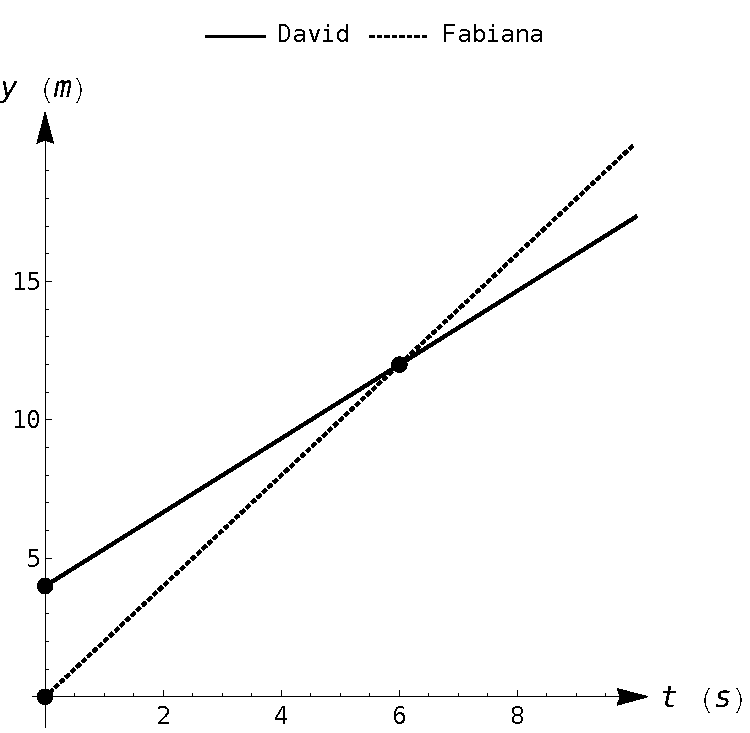
\includegraphics[scale=0.5]{fig_Systems_lin_eq_1}
	\caption{David and Fabiana's distances.}
	\label{fig_Systems_lin_eq_1}
\end{figure}


Each of the two lines has an equation. The line representing David appears to have $y$-intercept $(0,4)$ and slope $\frac{4}{3}$, so its equation is $y = \frac{4}{3}t+4$. The line representing Fabiana appears to have $y$-intercept $(0,0)$ and
slope $2$, so its equation is $y=2t$.	
We have the system of linear equations
\[\left\{ \begin{array}{l} y = \dfrac{4}{3}t+4 \\[0.2cm] y=2t.  \end{array} \right.  \]	

As we can see in Figure \ref{fig_Systems_lin_eq_1}, the graphs of the two equations cross at the point $(6,12)$. We refer to the point $(6,12)$ as the solution to this system of linear equations. To denote the solution set, we write	$\{(6,12)\}$. But it is much more valuable to interpret these numbers in context whenever possible: it took $6$ seconds for the two runners to meet up, and when they met they were $12$ meters up the track.
	
\end{example}

In Example \ref{graphing_syst_lin_eq_ex1}, we stated that the solution was the point  $(6,12)$. It makes sense to write this as an ordered pair when we are given a graph. In some cases when we have no graph, particularly when our variables are not $x$ and $y$, it might not be clear which variable comes first and we will not be able to write an ordered pair. Nevertheless, given the context we can write meaningful summary statements.	



\begin{example}\label{graphing_syst_lin_eq_ex2}
Solve the following system of equations by graphing.
\[\left\{ \begin{array}{rcl} x-3y & =& -12 \\ 2x+3y& =& 3  \end{array} \right.  \]	


\xhrulefill{gray}{2.5pt}Solution \xhrulefill{gray}{2.5pt}

Since both line equations are given in standard form, we will graph each one by finding the
intercepts. Recall that to find the $x$-intercept of each equation, replace $y$ with $0$ and solve for $x$. Similarly, to find the $y$-intercept of each equation, replace $x$ with $0$ and solve for $y$. For the first linear equation, we have:
\[ x = -12 \quad \text{ and } \quad y=4, \]
for the second linear equation:
\[ x = \dfrac{3}{2} \quad \text{ and } \quad y=1. \]
	
	
\begin{figure}[H]
	\centering
	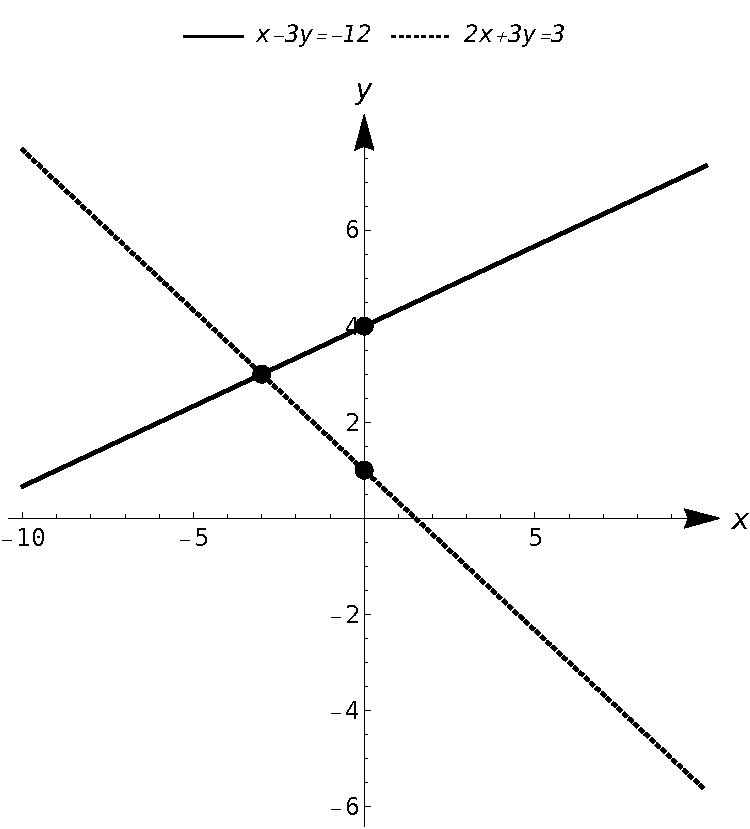
\includegraphics[scale=0.6]{fig_Systems_lin_eq_2}
	\caption{Graphs of $x-3y=-12$ and $2x+3y=3$.}
	\label{fig_Systems_lin_eq_2}
\end{figure}
	
It appears that the solution of the system of equations is the point of intersection of those two lines, which is $(-3,3)$. It is important to check if this is correct, because when making a hand-drawn graph, it would be easy to be off by a little bit. To check, we can substitute the values of $x$ and $y$ from the point $(-3,3)$ into each equation: 

\[ -3-9 \stackrel{\checkmark}{=} -12 \quad \text{ and } \quad  -6+9 \stackrel{\checkmark}{=} 3.  \]


We write the solution set as $\{(-3,3)\}$.

\end{example}


When we solve linear equations in one variable, we have two special cases. In one special case there is no solution and in the other case, there are infinitely many solutions. When solving systems of equations in two variables, we have two similar special cases.


%\begin{example}\label{graphing_syst_lin_eq_ex3}
Let us look at the graphs of two lines with the same slope, $y=2x-4$ and $y=2x+1$.
	
\begin{figure}[H]
	\centering
	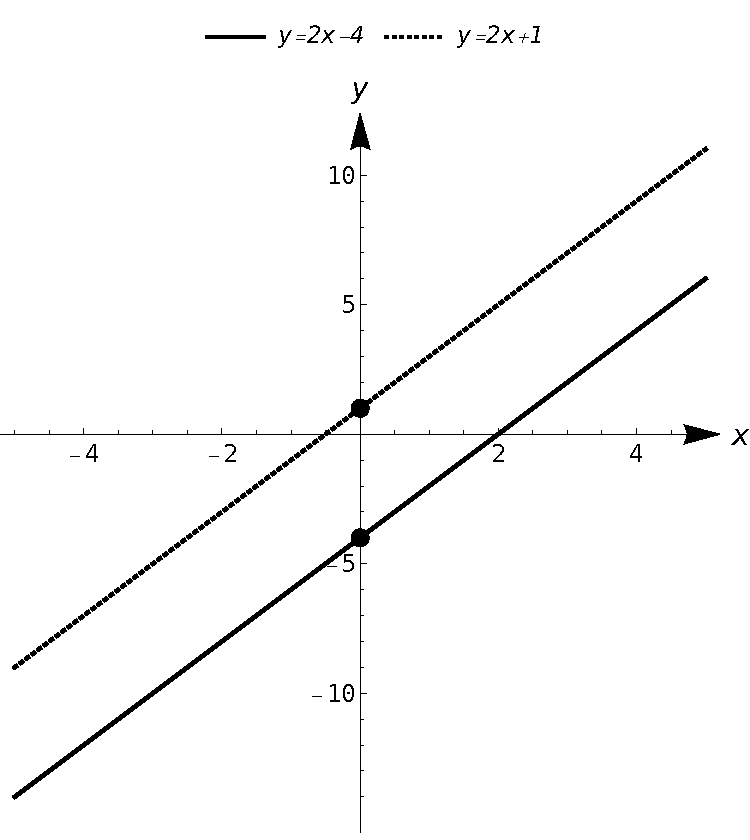
\includegraphics[scale=0.6]{fig_Systems_lin_eq_3}
	\caption{Graphs of $y=2x-4$ and $y=2x+1$.}
	\label{fig_Systems_lin_eq_3}
\end{figure}	

For this system of equations, what is the solution? Since the two lines have the same slope they are parallel lines and will never intersect. This means that there is no solution to this system of equations. We write the solution set as $\emptyset$ or $\{ \}$.	
	
%\end{example}



%\begin{example}\label{graphing_syst_lin_eq_ex4}
Next we will look at the other special case. We start with this system
of equations:
\[\left\{ \begin{array}{rcl} y & = & 2x-4 \\6x-3y  & = &  12. \end{array} \right.  \]	

To solve this system of equations, we want to graph each line. The first equation is in slope-intercept form and can be graphed easily using its slope of $2$ and its $y$-intercept of $(0,-4)$. The second equation, $6x-3y = 12$, can either be graphed by solving for $y$ and using the slope-intercept form or by finding the intercepts. If we use the intercept method, we find that this line has an $x$-intercept of $(2,0)$ and an $y$-intercept of $(0,-4)$. When we graph both lines we get Figure \ref{fig_Systems_lin_eq_4}.

\begin{figure}[h!]
	\centering
	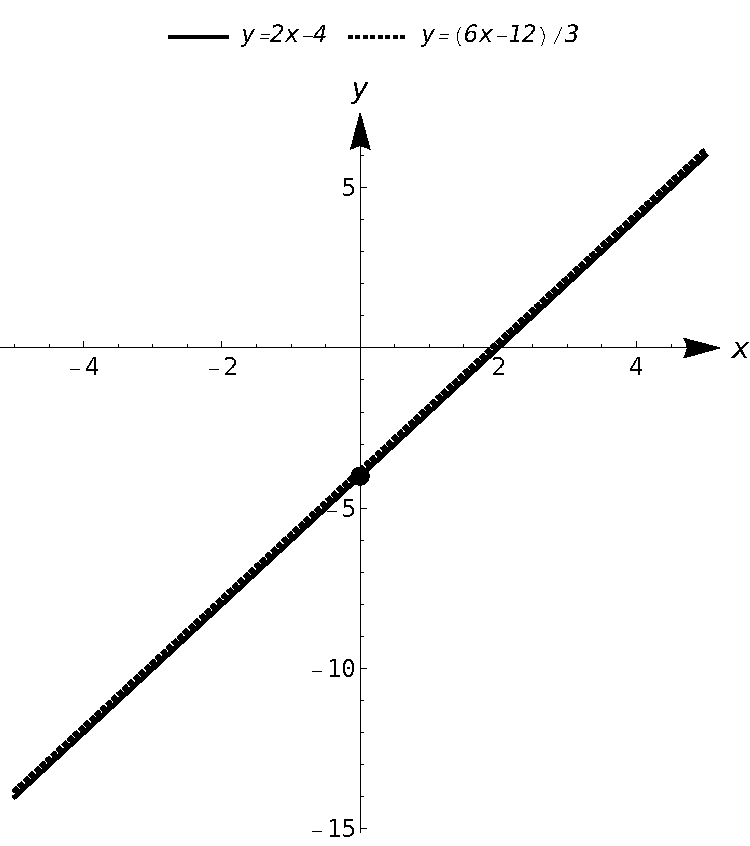
\includegraphics[scale=0.6]{fig_Systems_lin_eq_4}
	\caption{Graphs of $y=2x-4$ and $6x-3y = 12$.}
	\label{fig_Systems_lin_eq_4}
\end{figure}	

Now we can see these are actually the same line, or coinciding lines. To determine the solution to this system, we will note that they overlap everywhere. This means that we have an infinite number of solutions: all points that fall on the
line. It may be enough to report that there are infinitely many solutions. In order to be more specific, all we can do is say that any ordered pair $(x,y)$ satisfying the line equation is a solution. In set-builder notation (See Section \ref{sets}), we would write \\
$\{(x,y) \in \mathbb{R}^2 \, | \, y=2x-4  \}$.
	
%\end{example}


To summarize, there are three types of systems of two linear equations and their solution sets:
\begin{enumerate}
	\item If two linear equations have different slopes, the system has one solution.
	\item If two linear equations have the same slope with different $y$-intercepts, the system has no solution.
	\item If two linear equations have the same slope and the same $y$-intercept, the system has infinitely many solutions.
	This solution set consists of all ordered pairs on that line.
\end{enumerate}




\subsection{Solving systems of linear equations algebraically}  

\subsubsection{Substitution}  \label{syst_lin_eq_substitution}
In Section \ref{graphing_syst_lin_eq}, we focused on solving systems of equations by graphing. In addition to being time consuming, graphing can be an awkward method to determine the exact solution when it has large numbers or fractions. There are two symbolic methods for solving systems of linear equations, namely substitution and elimination. First, we will introduce one of them: \textbf{substitution} (\textit{substitutie})\index{substitution}.


%\subsubsection{Solving systems of equations using substitution}

\begin{example}\label{syst_lin_eq_substitution_ex1}
Solve the following systems of equations using substitution.
\begin{multicols}{2}
\begin{enumerate}
\item $\left\{ \begin{array}{rcl} x+2y &=& 8 \\[0.1cm] 3x - 2y &=& 8  \end{array} \right. $
\item $\left\{ \begin{array}{rcl} \dfrac{x}{3}-\dfrac{y}{2} &=& \dfrac{5}{6} \\[0.4cm] \dfrac{y}{2} + 1  &=& \dfrac{x}{4}  \end{array} \right. $
\end{enumerate}
\end{multicols}

\xhrulefill{gray}{2.5pt}Solution \xhrulefill{gray}{2.5pt}

\begin{enumerate}
\item The idea is to use one equation to find an expression that is equal to $x$ but, cleverly, does not use the variable $x$. Then substitute this for $x$ into the other equation. This leaves you with one equation that only has one variable. Looking at both equations, it will be easiest to solve for $x$ in the first equation:
\[x=8-2y. \]
Next, we replace $x$ by this expression in the second equation, giving us a linear equation in only one variable, $y$, that we may solve:
\begin{eqnarray*}
3x - 2y = 8 &\Rightarrow & 3(8-2y)-2y=8 \\ 
&\Leftrightarrow & 24-8y=8 \\ 
&\Leftrightarrow & y=2. 
\end{eqnarray*}

Now that we have the value for $y$, we need to find the value for $x$. We have already solved the first equation for $x$, so that is the easiest equation to use.
\[	x=8-2y \quad \Rightarrow \quad x = 8-2(2) = 4 \]

\item When a system of equations has fraction coefficients, it can be helpful to take steps that replace the fractions with whole numbers. With each equation, we may multiply each side by the least common multiple of all the denominators. In the first equation, the least common multiple of the denominators is 6, in the second equation this is 4, so
\[ \left\{ \begin{array}{rcl} \dfrac{x}{3}-\dfrac{y}{2} &=& \dfrac{5}{6} \\[0.4cm] \dfrac{y}{2} + 1  &=& \dfrac{x}{4}   \end{array} \right. \quad  \Leftrightarrow \quad \left\{ \begin{array}{rcl} 2x-3y & = & 5 \\[0.2cm] 2y+4 & = & x.  \end{array} \right.  \]
Now we have this system that is equivalent to the original system of equations, but there are no fraction coefficients. \\
The second equation is already solved for $x$, so we will substitute $x$ in the first equation with $2y+4$, and we have:
\begin{eqnarray*}
	2x-3y=5 &\Rightarrow & 2(2y+4)-3y=5  \\ 
	&\Leftrightarrow & y=-3. 
\end{eqnarray*}

And we have solved for $y$. To find $x$, we know $x=2y+4$, so we have $x=-2$.
\end{enumerate}
\end{example}


Let us see what happens when we use the substitution method when there are no or infinitely many solutions.

\begin{example} \label{syst_lin_eq_substitution_ex2}
Solve the following systems of equations using substitution.
\begin{multicols}{2}
\begin{enumerate}
\item $\left\{ \begin{array}{rcl} 2x-1&=&y \\ 4x-2y&=&3  \end{array} \right. $
\item $\left\{ \begin{array}{rcl} 2x-1&=&y  \\ 4x-2y&=&2  \end{array} \right. $
\end{enumerate}
\end{multicols}


\xhrulefill{gray}{2.5pt}Solution \xhrulefill{gray}{2.5pt}

\begin{enumerate}
\item Since the first equation is already solved for $y$, we will substitute $ 2x-1$ for $y$ in the second equation, and we have:

\begin{eqnarray*}
	4x-2y=3 &\Rightarrow & 4x - 2(2x-1) = 3  \\ 
	&\Leftrightarrow & 2=3. 
\end{eqnarray*}

Even though we were only intending to substitute away $y$, we ended up with an equation where there are no variables at all. This will happen whenever the lines have the same slope. This tells us the system represents either parallel or coinciding lines. Since $2=3$ is false no matter what values $x$ and $y$ might be, there can be no solution to the system. So the lines are parallel and distinct.

\item We substitute $2x-1$ for $y$ in the second equation and we have:
\begin{eqnarray*}
	4x-2y=2 &\Rightarrow & 4x - 2(2x-1) = 2  \\ 
	&\Leftrightarrow & 2=2. 
\end{eqnarray*}

Even though we were only intending to substitute away $y$, we ended up with an equation where there are no variables at all. This will happen whenever the lines have the same slope. This tells us the system represents either parallel or coinciding lines. Since $2=2$ is true no matter what values $x$ and $y$ might be, the system equations are true no matter what $x$ is, as long as $y=2x-1$. So the lines coincide. This means that these two different linear equations are, in fact, equivalent.  
One way to describe the solution set to this system is to use the set-builder method and write $\{(x,y) \in \mathbb{R}^2 \, | \, 4x-2y = 2\}$.  \\
While this is correct, we take this opportunity to introduce the notion of a \index{parametric solution} \index{system of equations ! parametric solution}\textbf{parametric solution to a system} (\textit{parametrische oplossing van een stelsel}).  Our first step is to solve one of the two equations for one of the variables, say $y = 2x-1$.  For each value of $x$, the formula $y = 2x-1$ determines the corresponding $y$-value of a solution.  Since we have no restriction on $x$, it is called a \index{system of equations ! free variable} \index{free variable} \textbf{free variable} (\textit{vrije variabele}).  We let $x=t$, a so-called 'parameter', and get $y = 2t-1$. Our set of solutions can then be described as $\left\{ \left(t, 2t-1\right) \, | \, t \in \mathbb{R}\right\}$. Note that we could have just as easily chosen to solve $y=2x-1$ for $x$.  There is no one correct way to parameterize the solution set, which is why it is always best to check your answer. For that purpose, we claim that for any real number $t$, the pair $\left(t, 2 t - 1\right)$ satisfies both equations.  Substituting $x = t$ and $y =  2 t - 1$ into $4x-2y=2$ gives $4t - 2\left(2t-1\right) = 2$.  Simplifying, we get $4t - 4t + 2 = 2$, which is always true.  

Geometrically, $y=2x-1$ and $4x-2y=2$ are the same line, which means that they intersect at every point on their graphs. Every point on the line is a solution to the system, so the system has infinitely many solutions. The reader is encouraged to think about how our parametric solution says exactly that.


\end{enumerate}

\end{example}

It is clear that some systems of equations have solutions, and some do not. Those which have solutions are called \index{consistent system} \index{system of equations ! consistent} \textbf{consistent} (\textit{oplosbaar}), those with no solution are called \index{inconsistent system} \index{system of equations ! inconsistent} \textbf{inconsistent} (\textit{niet oplosbaar}). We also distinguish the two different types of behavior among consistent systems. Those which admit free variables are called \index{system of equations ! dependent} \index{dependent system} \textbf{dependent} (\textit{afhankelijk});  those with no free variables are called \index{system of equations ! independent} \index{independent system} \textbf{independent} (\textit{onafhankelijk}). In the case of systems of linear equations, regardless of the number of equations or variables, consistent independent systems have exactly one solution.  



\subsubsection{Elimination}\label{syst_lin_eq_elimination}
In this section, we will learn a second symbolic method for solving systems of linear equations.


\begin{example}\label{syst_lin_eq_elimination_ex1}
Solve the following system of equations.

\[ \left\{ \begin{array}{l} 5x+4y=-7 \\ 5x+2y=-1  \end{array} \right.  \]


\xhrulefill{gray}{2.5pt}Solution \xhrulefill{gray}{2.5pt}

We could also solve this system by substitution, but there is an easier method. If
we subtract the left sides from the two equations, it should equal the difference of the right sides. So we have
\[ 2y=-6.  \]

Note that the variable $x$ is eliminated. This happened because $5x$ and $-5x$ were perfectly in shape to cancel each other out. With only one variable left, it does not take much to finish: $y=-3$. To finish solving this system of equations, we need the value of $x$. For now, an easy way to find $x$ is to substitute our value of $y$ into one of the original equations:
\[ 5x + 2y = -1 \quad \Rightarrow  \quad 5x + 2(-3) = -1  \quad \Leftrightarrow  \quad x = 1. \]
The solution to the system is $(1,-3)$.

\end{example}



This method for solving the system of equations in Example \ref{syst_lin_eq_elimination_ex1} worked because $5x$ and $5x$ substract to zero.
Once the $x$-terms were eliminated we were able to solve for $y$. This method is called the \textbf{elimination method} (\textit{eliminatiemethode}). Some textbooks call it the \textbf{addition method} (\textit{combinatiemethode}). \\


If neither variable can be immediately eliminated, we can still use this method but it will require that we first adjust one or both of the equations. Let us look at an example where we need to adjust one of the equations.




\begin{example}\label{syst_lin_eq_elimination_ex2}
Solve the following system of equations.
	
\[ \left\{ \begin{array}{rcl} 3x - 4y &=& 2 \\[0.1cm] 5x + 8y &= &18  \end{array} \right.  \]
	
	
\xhrulefill{gray}{2.5pt}Solution \xhrulefill{gray}{2.5pt}
	
To start, we want to see whether it will be easier to eliminate $x$ or $y$. We see that the
coefficients of $x$ in each equation are $3$ and $5$, and the coefficients of $y$ are $-4$ and $8$. Because $8$ is a multiple of $4$ and the coefficients already have opposite signs, the variable $y$ will be easier to eliminate. To eliminate the $y$-terms, we will multiply each side of the first equation by $2$ so that we will have $-8y$.
We can call this process scaling the first equation by $2$. \\
We now have an equivalent system of equations where the $y$-terms can be eliminated:
\[ \left\{ \begin{array}{rcl} 6x-8y&=&4 \\[0.1cm] 5x+8y&=&18.  \end{array} \right. \] 
We add the two equations, which give
\[ x=2. \]
To solve for $y$, we will substitute $2$ for $x$ into either of the original equations or the new one. We will use the original first equation, $3x-4y=2$, so we have:
\[ 6-4y=2 \quad \Leftrightarrow \quad y=1. \]	
The solution to this system is  $(2,1)$ and the solution set is $\{(2,1)\}$.	
	
\end{example}

Sometimes a system of equations has no solutions at all, and sometimes the solution set is infinite with all of the points on one line satisfying the equations. Let us again see what happens when we use the elimination method on each of the special cases.



\begin{example} \label{syst_lin_eq_elimination_ex3}
Solve the following systems of equations using substitution.
\begin{multicols}{2}
\begin{enumerate}
	\item $\left\{ \begin{array}{rcl} 3x+4y&=&5 \\[0.1cm] 6x+8y&=&10  \end{array} \right. $
	\item $\left\{ \begin{array}{rcl}10x+6y&=&9 \\[0.1cm] 25x+15y&=&4  \end{array} \right. $
\end{enumerate}
\end{multicols}
	
	
\xhrulefill{gray}{2.5pt}Solution \xhrulefill{gray}{2.5pt}
	
\begin{enumerate}
\item To eliminate the $x$-terms, we multiply each term in the first equation by $-2$, and we have:
\[ \left\{ \begin{array}{rcl} -6x-8y&=&-10 \\[0.1cm] 6x+8y&=&10.  \end{array} \right. \]
We might notice that the equations look very similar. Adding the respective sides of the equation, we have:
\[ 0=0. \]
Both of the variables have been eliminated. Since the statement $0=0$ is true no matter what $x$ and $y$ are, the solution set is infinite. Specifically, you just need any $(x,y)$ satisfying one of the two equations, since the two equations represent the same line. We can write the solution set as $\{ (x,y) \in \mathbb{R}^2 \, | \, 3x+4y=5 \}$.		
		
	
\item To eliminate the $x$-terms, we will scale the first equation by $-5$ and the second by $2$:
\[ \left\{ \begin{array}{rcl} -50x-30y&=&-45 \\ 50x+30y&=&8.  \end{array} \right. \]
Adding the respective sides of the equation, we have:
\[ 0=-37. \]
Both of the variables have been eliminated. In this case, the statement $0=-37$ is just false, no matter what $x$ and $y$ are. This tells us that it is impossible to find a pair $(x,y)$ which satisfies both equations; in other words, the system has no solution. 		
		
\end{enumerate}
	
\end{example}

In every example so far from this section, both equations were in standard form, $ax + by=c$. And all of the coefficients were integers. If none of the coefficients are equal to $1$ then it is usually easier to use the elimination method, because otherwise you will probably have some fraction arithmetic to do in the middle of the substitution method. If there is a coefficient of $1$, then it is a matter of preference.



\begin{example} \label{syst_lin_eq_elimination_ex4} 
Solve the following system of equations.

\[\left\{ \begin{array}{rcl} x - y &=& 0 \\ x + y &=& 2 \\ -2x + y &=& -2 \end{array} \right. \]


\xhrulefill{gray}{2.5pt}Solution \xhrulefill{gray}{2.5pt}

We can begin to solve this system by adding the first two equations:  

\setlength{\extrarowheight}{2pt}
\[ \begin{array}{lrcr} & x - y & = & 0  \\ + & (x + y & = & 2 ) \\ \hline  & 2x & = & 2 \end{array}\]  
\setlength{\extrarowheight}{0pt}

which gives $x = 1$.  Substituting this into the first equation gives $1 - y = 0$ so that $y = 1$.  We seem to have determined a solution to our system, $(1,1)$.  While this checks in the first two equations, when we substitute $x=1$ and $y=1$ into the third equation, we get $-2(1) + (1) = -2$ which simplifies to the contradiction $-1 = -2$.  Graphing the lines $x-y=0$, $x+y = 2$, and $-2x+y=-2$, we see that the first two lines do, in fact, intersect at $(1,1)$, however, all three lines never intersect at the same point simultaneously, which is what is required if a solution to the system is to be found.

\begin{figure}[H]
	\centering
	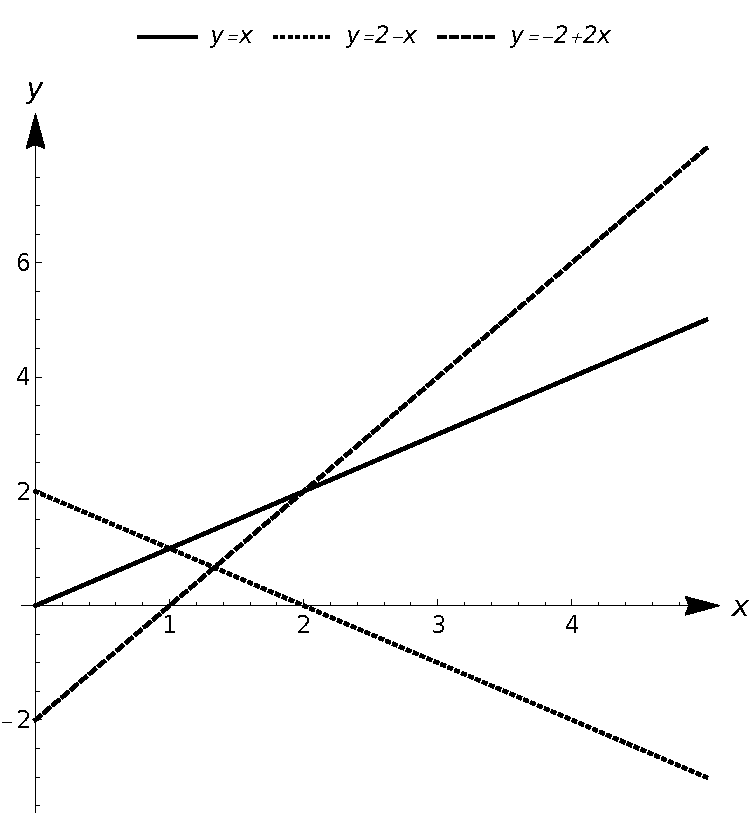
\includegraphics[scale=0.6]{fig_Systems_lin_eq_5}
	\caption{Graphs of $x-y=0$, $x+y=2$ and $-2x+y = -2$.}
	\label{fig_Systems_lin_eq_5}
\end{figure}


\end{example}


The system in Example \ref{syst_lin_eq_elimination_ex4} is called \index{system of equations ! overdetermined} \index{overdetermined system} \textbf{overdetermined} (\textit{overbepaald}), since we have more equations than variables. Not surprisingly, a system with more variables than equations is called \index{system of equations ! underdetermined} \index{underdetermined system} \textbf{underdetermined} (\textit{onderbepaald}).  While the system in Example \ref{syst_lin_eq_elimination_ex4} is overdetermined and inconsistent, there exist overdetermined consistent systems (both dependent and independent) and we leave it to the reader to think about what is happening algebraically and geometrically in these cases.  Likewise, there are both consistent and inconsistent underdetermined systems. But a consistent underdetermined system of linear equations is necessarily dependent.

\smallskip



%We have seen plenty of instances of the second and third moves in Theorem \ref{equationmoves} when we solved the systems Example \ref{reviewsubelim}. The first move, while it obviously admits an equivalent system, seems silly.  Our perception will change as we consider more equations and more variables in this, and later sections.
%
%\smallskip

In the last example, we consider a system of linear equations in three variables.


\begin{example} \label{syst_lin_eq_elimination_ex5} 
Solve the system of equations 
\[ \left\{ \begin{array}{rcl} x-\dfrac{1}{3}y+\dfrac{1}{2}z &=& 1 \\[0.4cm]
y - \dfrac{1}{2} z &=& 4 \\[0.4cm]
z &=& -1. \\ \end{array} \right.\]  

\xhrulefill{gray}{2.5pt}Solution \xhrulefill{gray}{2.5pt}
	

Clearly $z = -1$, and we substitute this into the second equation $y - \frac{1}{2} (-1) = 4$ to obtain $y = \frac{7}{2}$.  Finally, we substitute $y = \frac{7}{2}$ and $z=-1$ into the first equation to get $x - \frac{1}{3}\left(\frac{7}{2}\right) + \frac{1}{2}(-1) = 1$, so that $x = \frac{8}{3}$.  The reader can verify that these values of $x$, $y$ and $z$ satisfy all three original equations.  It is tempting for us to write the solution to this system by extending the usual $(x,y)$ notation to $(x,y,z)$ and list our solution as $\left(\frac{8}{3},\frac{7}{2},-1\right)$.  The question quickly becomes what does an `ordered triple' like $\left(\frac{8}{3},\frac{7}{2},-1\right)$ represent?  Just as ordered pairs are used to locate points on the two-dimensional plane, ordered triples can be used to locate points in space. Moreover, just as equations involving the variables $x$ and $y$ describe graphs of one-dimensional lines and curves in the two-dimensional plane, equations involving variables $x$, $y$, and $z$ describe objects called \textbf{surfaces} (\textit{oppervlakken}) in three-dimensional space.  Each of the equations in the above system can be visualized as a plane situated in three-dimensional space.  Geometrically, the system is trying to find the intersection, or common point, of all three planes. It turns out that any two of these planes intersect in a line, so our intersection point is where all three of these lines meet. In fact, these lines are described by the parametric solutions to the systems formed by taking any two of these equations by themselves.

%\centerline{\includegraphics[width=3in]{./MatricesGraphics/3planes01.jpg}}

We note the reason it was so easy to solve is that the third equation is solved for $z$, the second equation involves only $y$ and $z$, and since the coefficient of $y$ is $1$, it makes it easy to solve for $y$ using our known value for $z$.  Lastly, the coefficient of  $x$ in the first equation is $1$ making it easy to substitute the known values of $y$ and $z$ and then solve for $x$.  


\end{example}








\section{Systems of linear inequalities}\label{syst_lin_ineq}
%https://www.universalclass.com/articles/math/algebra/solving-systems-of-linear-inequalities.htm \\
%
%
%https://www.mathplanet.com/education/algebra-1/systems-of-linear-equations-and-inequalities/systems-of-linear-inequalities

\textbf{A system of linear inequalities in two variables} (\textit{stelsel van lineaire ongelijkheden in twee veranderlijken}) consists of at least two linear inequalities in the same variables. The solution of a linear inequality is the ordered pair that is a solution to all inequalities in the system and the graph of the linear inequality is the graph of all solutions of the system. \\



\subsection{Graphing systems of linear inequalities} \label{graphing_syst_lin_ineq}
One linear inequality in two variables divides the plane into two half-planes. To graph the inequality, graph the equation of the boundary. To graph a linear inequality in two variables $x$ and $y$, first get $y$ alone on one side. Then consider the related equation obtained by changing the inequality sign to an equality sign. The graph of this equation is a line.\\

If the inequality is strict ($<$ or $>$), graph a dashed line to indicate that the boundary is not part of the solution. If the inequality is not strict ($\leq$ or $\geq$ ), a solid line is used because the boundary is included in the solution. Finally, pick one point that is not on either line ($(0,0)$ is usually the easiest) and decide whether these coordinates satisfy the inequality or not. If they do, shade the half-plane containing that point. If they don't, shade the other half-plane. Unless you are graphing a vertical line the sign of the inequality will let you know which half-plane to shade.  If the symbol $\geq$ or $>$ is used, shade above the line. If the symbol $\leq$ or $<$ is used shade below the line. For a vertical line, larger solutions are to the right and smaller solutions are to the left. A system of two or more linear inequalities can divide the plane into more complex shapes. \\

Graph each of the inequalities in the system in a similar way. The solution of the system of inequalities is the intersection region of all the solutions in the system.

\begin{example}\label{graphing_syst_lin_ineq_ex1}
Solve the following systems of inequalities by graphing.
\begin{multicols}{2}
\begin{enumerate}
\item $\left\{ \begin{array}{rcl} y &\leq& x-2 \\ y &>& -3x+5  \end{array} \right. $
\item $\left\{ \begin{array}{rcl} 2x+3y &\geq& 12 \\ 8x-4y &>& 1 \\ x &<& 4  \end{array} \right. $
\end{enumerate}
\end{multicols}

%https://www.varsitytutors.com/hotmath/hotmath_help/topics/graphing-systems-of-linear-inequalities -> OK

\xhrulefill{gray}{2.5pt}Solution \xhrulefill{gray}{2.5pt}

\begin{enumerate}
\item First, we graph the inequality  $y \leq x-2$. The related equation is $y=x-2$. Since the inequality is not a strict one, the border line is solid. We consider the point $(0,0)$ that is not on the line, and substitute this in the inequality $y \leq x-2$: $0 \leq 0-2 $. This is false. So, the solution does not contain the point $(0,0)$. We shade the lower half of the line. Similarly, we draw a dashed line for the related equation of the second inequality $y > -3x+5$ which has a strict inequality. The point $(0,0)$ does not satisfy the inequality, so we shade the half that does not contain the point $(0,0)$. 
The solution of the system of inequalities is the intersection region of the solutions of the two inequalities (Figure \ref{fig_Systems_lin_eq_6}).
\begin{figure}[H]
	\centering
	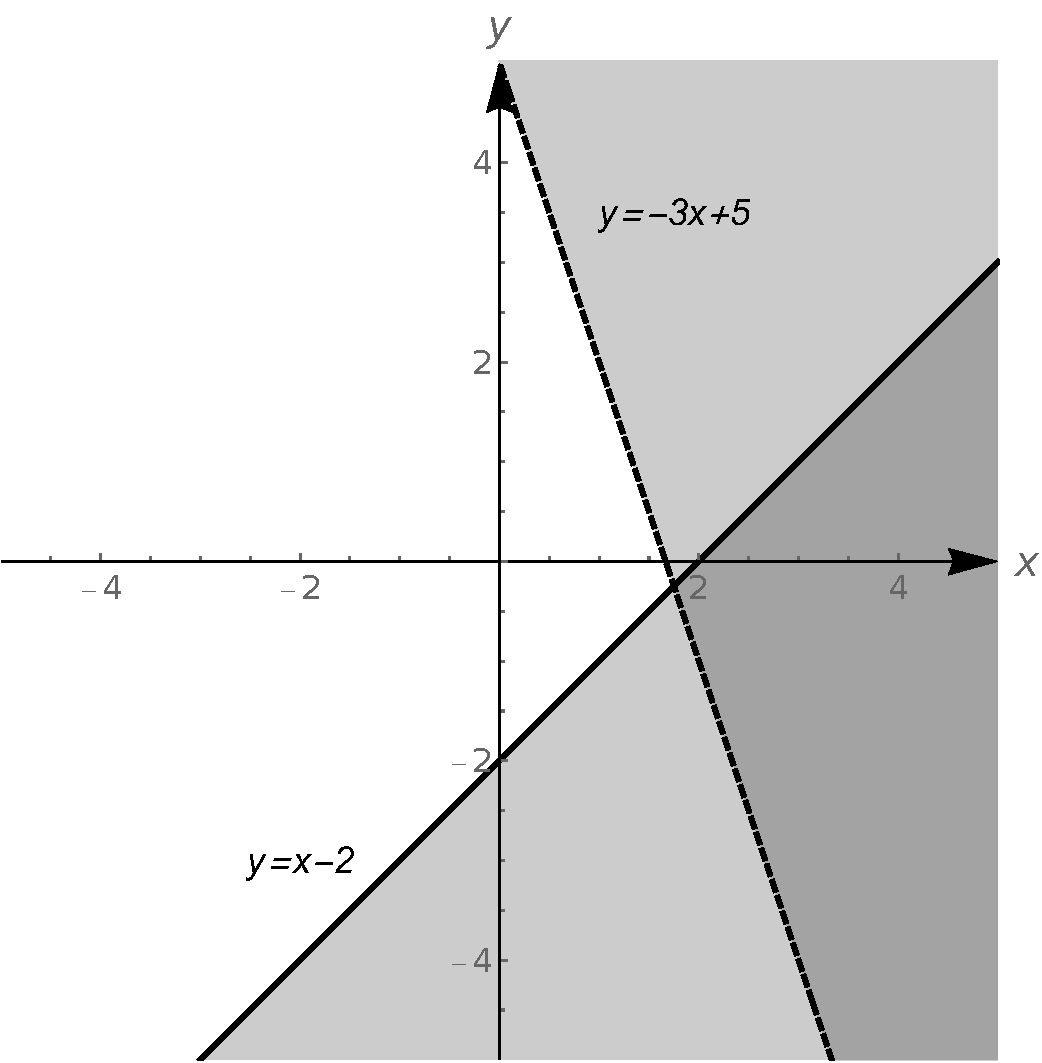
\includegraphics[scale=0.4]{fig_Systems_lin_eq_6}
	\caption{Solution of the system of inequalities is the intersection region of the solutions of the two inequalities $y \leq x-2$ and $y > -3x+5$.}
	\label{fig_Systems_lin_eq_6}
\end{figure}

\item Rewrite the first two inequalities with $y$ alone on one side.
\[\left\{ \begin{array}{rcl} 2x+3y &\geq& 12 \\ 8x-4y &>& 1 \\ x &<& 4  \end{array} \right. \quad \Leftrightarrow \quad \left\{ \begin{array}{rcl} y &\geq& -\dfrac{2}{3}x+4 \\ y&<&2x -\dfrac{1}{4} \\ x &<& 4  \end{array} \right. \]
Now, we graph $y =-\frac{2}{3}x+4$ and $y=2x -\frac{1}{4}$. The point $(0,0)$ does not satisfy the inequalities, so we shade the half that does not contain the point $(0,0)$. 
Similarly, we draw a dashed vertical line $x=4$ which is the related equation of the third inequality $x<4$ and shade the half that contains $(0,0)$.
The solution of the system of inequalities is again the intersection region of the solutions of the three inequalities (Figure \ref{fig_Systems_lin_eq_7}).
\begin{figure}[H]
	\centering
	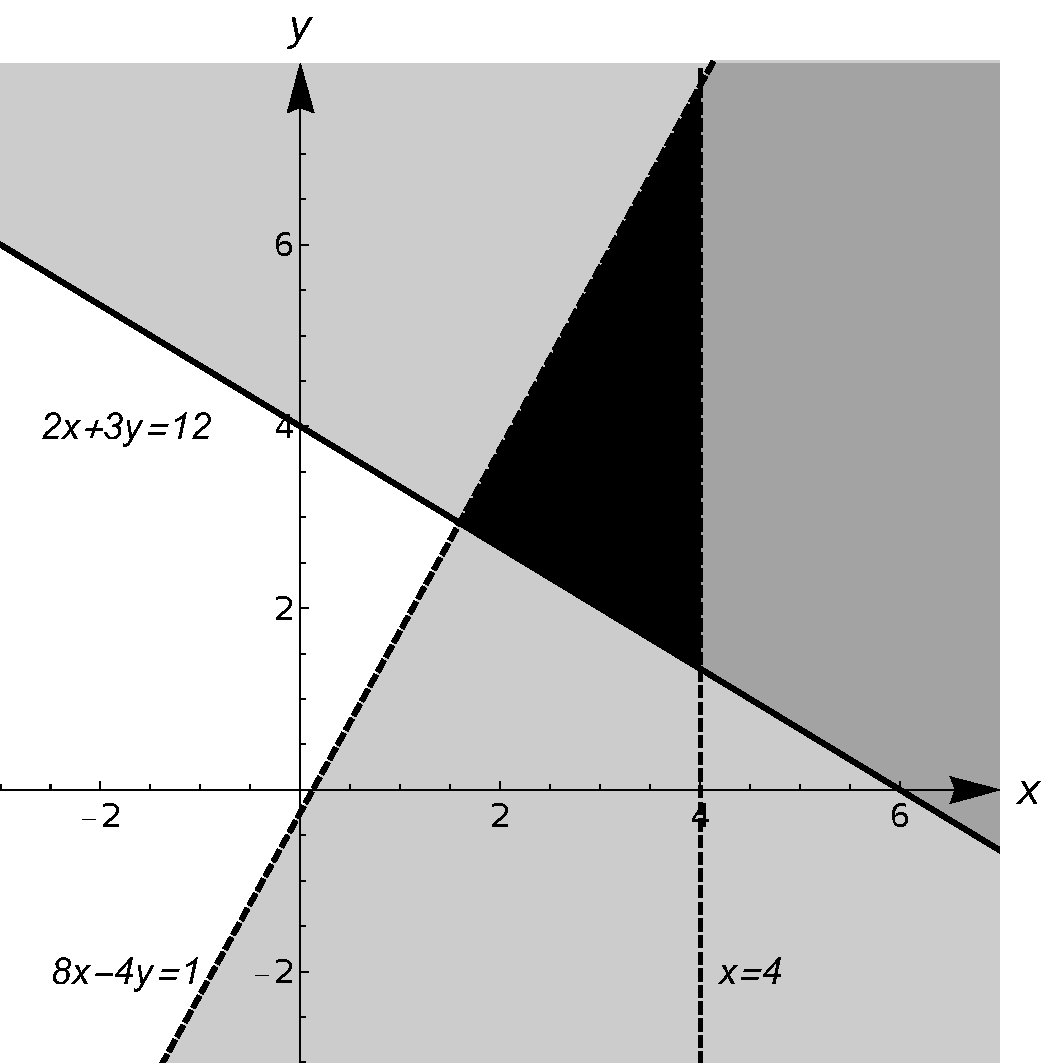
\includegraphics[scale=0.4]{fig_Systems_lin_eq_7}
	\caption{Solution of the system of inequalities is the intersection region of the solutions of the three inequalities $2x+3y\geq 12$, $8x-4y> 1$ and $x < 4$.}
	\label{fig_Systems_lin_eq_7}
\end{figure}


\end{enumerate}

\end{example}


\subsection{Solving systems of linear inequalities algebraically}\label{syst_lin_ineq_alg}
The techniques for solving systems of linear inequalities differ from those for linear equations because the inequality signs do not allow us to perform substitution as we do with equations. Nevertheless, we can still solve these problems. When solving systems of linear inequalities, we solve each inequality separately and find the common values between the two (or more) inequalities. 

\begin{example}
Solve the following systems of inequalities algebraically.	
	
\begin{enumerate}
	\item $ \left\{\begin{array}{rcl}
	2(4x+1) & \geq &5x+8 \\
	2(3x+2) & >         &5(3x-10)
	\end{array}\right. $	
	
	\item $\left\{\begin{array}{rcl}
		\dfrac{x-1}{x+2}  & <	&\dfrac{x+1}{x+4} \qquad  (x\neq -2 \text{ and } x\neq -4) \\[0.1cm]
		5x-2		  &\geq &2x+1
	\end{array}\right.	$
\end{enumerate}	

\ifvc\pagebreak\fi
\xhrulefill{gray}{2.5pt}Solution \xhrulefill{gray}{2.5pt}	
	
	
\begin{enumerate}
\item
 
We first solve the first inequality and rewrite these with $x$ alone on one side.
\[\begin{array}{rcrcl}
	2(4x+1) \geq 5x+8 	&\Leftrightarrow& 8x+2 & \geq &  5x+8 \\
	&\Leftrightarrow& 3x & \geq & 6 \\
	&\Leftrightarrow& x & \geq & 2
\end{array}
\]

Similarly, we solve the second inequality.
\[\begin{array}{rcrcl}
	2(3x+2) >   5(3x-10)	&\Leftrightarrow& 6x+4 & > &15x-50 \\
	&\Leftrightarrow& -9x & > & -54\\
	&\Leftrightarrow& x & < &6
\end{array}
\]


The solution set exists of the common values between the two inequalities:
\[ \{x\in\mathbb{R} \, | \, x\geq 2\} \cap \{x\in \mathbb{R} \, | \,  x<6\}=\{x\in \mathbb{R}\,  | \,  2\leq x<6\}.\]

\item To solve the first, rational, inequality, we first put both fractions on the left-hand side and make the denomenators the same. 
\[\begin{array}{rcrcl}
	\dfrac{x-1}{x+2}-\dfrac{x+1}{x+4} < 0	& \Leftrightarrow& \dfrac{(x-1)(x+4)-(x+1)(x+2)}{(x+2)(x+4)} & < &0 \\[0.4cm]
	& \Leftrightarrow& \dfrac{-6}{(x+2)(x+4)} & < &0  \\[0.4cm]
	& \Leftrightarrow& \dfrac{6}{(x+2)(x+4)} & > & 0 \\[0.4cm]
	& \Leftrightarrow& (x+2)(x+4) & > & 0
\end{array}
\]
We define the zeros from the polynomial $(x+2)(x+4)$ and use these points to divide the number line into intervals. Then we determine the sign of the polynomial on each interval.
\[ \begin{array}{c|ccccc}
x     &      &-4     &	    &-2      & \\
\hline
x+2   &-     &	     &-     &0	     &+ \\
x+4   &-     &0      &+     &	     &+ \\
\hline
(x+2)(x+4) &+  &|    &-     &|	     &+
\end{array}\] 

The solution set is
\[\{x \in \mathbb{R}\, | \, x<-4  \, \vee \, x>-2\}. \]


We rewrite the second inequality with $x$ alone on one side.
\[ 5x-2 \geq 2x+1 \quad \Leftrightarrow \quad 3x \geq 3  \quad \Leftrightarrow \quad x\geq 1 \]
The solution set is
\[\{x\in \mathbb{R}\, |\, x \geq 1\}. \]


The solution set exists again of the common values between the two inequalities:
\[ \{ x\in \mathbb{R}\, |\, x<-4 \, \vee \, x>-2\} \cap \{x \in \mathbb{R}\, | \, x\geq 1\} =\{x\in \mathbb{R} \, | \, x\geq 1\}. \]


\end{enumerate}	

\end{example}



\section{Exercises}
\begin{enumerate}

\item Bepaal algebra\"isch en grafisch de oplossingsverzameling van de onderstaande stelsels.
\begin{multicols}{2}
\begin{enumerate}
\item $\left\{\begin{array}{l}
2x - 5y = 19 \\
x - 6y = 20
\end{array} \right. $
\item []
\item $\left\{\begin{array}{l}
x + 2y = 23 \\
13x - 11y = 3
\end{array} \right. $
\item []
\item $\left\{\begin{array}{l}
8x + y = 25 \\
12x = 32 + 4y
\end{array} \right. $
\item []
\item $\left\{\begin{array}{l}
8(x + 1) = 7(y - 1) - 80 \\
14x = 26y - 180
\end{array} \right. $
\item []
\item $\left\{\begin{array}{l}
2x + 3y = 13 \\
-3x + 4y = 23
\end{array} \right. $
\item []
\item $\left\{\begin{array}{l}
-x + 2y = -1 \\
3x -6y = 3
\end{array} \right. $
\item []
\item $\left\{\begin{array}{l}
4x + y = 10 \\
5x -3y = 21
\end{array} \right. $


\item []
\item $\left\{\begin{array}{l}
3x - y = 4 \\
x -11y = -16 \\
x+5y = 10 \\
3x-17y=-22
\end{array} \right. $

\end{enumerate}
\end{multicols}


\item Bepaal algebra\"isch de oplossingsverzameling van de onderstaande stelsels.
\begin{multicols}{2}
\begin{enumerate}
\item $\left\{\begin{array}{l}
x + y - 3z = 5 \\
3x + 2y - 9z = 10
\end{array} \right. $
\item []
\item $\left\{\begin{array}{l}
x + 2y + 3z = 0 \\
3x + 2y + z = 0
\end{array} \right. $
\item []
\item $\left\{\begin{array}{l}
2x + y - z = 9 \\
x + 3y + z = 6 \\
5x - y + 2z = -6
\end{array} \right. $
\item []
\item $\left\{\begin{array}{l}
x + y + z = 7 \\
2x - 3y + 5z = 8 \\
x - 4y + 4z = 2
\end{array} \right. $
\item []
\item $\left\{\begin{array}{l}
x - 4y + 6z = 14 \\
5x + 2y + 3z = 23 \\
2x + 6y - 6z = -3
\end{array} \right. $
\item []
\item $\left\{\begin{array}{l}
x + y - 5z = 11 \\
x - y + z = -7 \\
2x + y = 6 \\
y - z = 7
\end{array} \right. $

\item []
\item $\left\{\begin{array}{l}
x + y + z = 6 \\
-3x +2 y + z = -1 \\
x - 4y + 2z = 4
\end{array} \right. $

\item []
\item $\left\{\begin{array}{l}
x -2y + 3z = 0 \\
2x + y + z = 0 \\
4x +7y -3z = 0
\end{array} \right. $

\item []
\item $\left\{\begin{array}{l}
x +y+z = 4 \\
x-y+2z=0 
\end{array} \right. $


\end{enumerate}
\end{multicols}

\item Bepaal grafisch de oplossingsverzameling van de onderstaande stelsels ongelijkheden.
\begin{multicols}{2}
\ben
\item $\left\{\begin{array}{rcl}
 x+3y &<&7 \\ -2x+4y &\geq& 2
\end{array}\right. $ 

\item $\left\{\begin{array}{rcl}
 x+2y &\leq& 2 \\2x+4y &\geq& 8
 \end{array}\right.$

\item $\left\{\begin{array}{rcl}
 x-y &>& 2 \\ 2x-2y &<& 6
 \end{array}\right.$

\item $\left\{\begin{array}{rcl}
 x+y &>&2 \\ 4x+4y &>& 16
 \end{array}\right.$

\item $\left\{\begin{array}{rcl}
 x+2y &\leq& 2 \\ -x+2y &<& 2 \\ 2y &<& 1
 \end{array}\right. $
\item []

\item $\left\{\begin{array}{rcl}
 x+3y &<&3 \\ 2x+4y & <& 2 \\ x-y &<& 0
 \end{array}\right. $
\item []

\item $\left\{\begin{array}{rcl}
 x-y &\geq& 0 \\y+3 &>& 0 \\x-2 &<&0
 \end{array}\right.$
\een
\end{multicols}

\item Een motorijder rijdt $40\, \mathrm{km}$ per uur op de vlakke gedeelten van een weg,
$60 \, \mathrm{km}$ op de dalende en $28 \, \mathrm{km}$ op de stijgende.  Hij reed in $8\, \mathrm{u} \,03 \,\mathrm{min}$ van
$A$ naar $B$, en in $8\, \mathrm{u} \,27 \,\mathrm{min}$ van $B$ naar $A$. Hoeveel kilometers vlak,
stijgend en dalend terrein zijn er van $A$ naar $B$ als de afstand
$AB$ $321\, \mathrm{km}$ is ?

\item Water vloeit van reservoir $A$ naar reservoir $B$ met een snelheid van 2 liter per minuut. Toen de kraan
opengezet werd, bevatten beide reservoirs 15 liter. Na hoeveel tijd zal de inhoud van $B$ het kwadraat zijn van die van $A$?


\item Een leraar laat 16 vraagstukken in zijn klas oplossen. Hij zal 5 punten geven voor elke goede oplossing en 3 punten aftrekken voor een foute oplossing. Hoeveel goede oplossingen had een leerling die noch wint, noch verliest?

\item Een zeker bedrag wordt tussen twee personen verdeeld. Als de eerste persoon 60 euro en nog 3/7 van het overschot neemt, dan heeft hij de helft meer dan de tweede. Hoe groot was het te verdelen bedrag?

\item Van drie kapitalen is het tweede het dubbel van het eerste en het derde het
drievoud van het tweede. De kapitalen stonden respectievelijk 4 jaar tegen $5\%$, 3 jaar 9
maand tegen $4\%$ en 2 jaar 8 maand tegen $3\%$ uit. Ze brachten samen 2646 euro intrest op. Bepaal ieders kapitaal en zijn intrest.

\item Twee vrienden vertrekken om 8 uur 's morgens, de ene uit Gent, de andere uit Antwerpen, en fietsen elkaar tegemoet. De eerste legt $18\, \mathrm{km}$ per uur af, de tweede $15\, \mathrm{km}$ per uur. De afstand Gent-Antwerpen is 55 km. Waar en wanneer zullen ze elkaar ontmoeten?

%\item Hoe laat is het tussen 5 en 6 uur als de wijzers van een klok:
%\ben
%\item elkaar bedekken,
%\item in elkaars verlengde staan,
%\item loodrecht op elkaar staan?
%\een

\item Drie werkmannen verdienen samen 500 euro per dag voor een werk dat ze alleen in respectievelijk 27, 30, 45 dagen kunnen afmaken. Bepaal ieders dagloon.

\item Als twee personen samenwerken voltooien ze een werk in 6 uren. Deden ze na elkaar de helft van het werk, dan was de totale tijd $12\, \mathrm{u}\, 30 \, \mathrm{min}$. In hoeveel tijd kan elke persoon alleen het werk afmaken?

\item Een erfenis van 60 000 euro moet in gelijke delen onder een aantal personen verdeeld worden. Twee erfgenamen worden uitgesloten en zo krijgt elke overblijvende erfgenaam 5000 euro meer. Hoeveel erfgenamen waren er oorspronkelijk?


\item Een kapitaal van 5000 euro wordt gedurende twee jaar tegen een zeker intrestpercentage uitgezet.
Achteraf wordt dit kapitaal vermeerderd met de verworven intrest opnieuw uitgezet tegen een percentage dat $1\%$ hoger is. De jaarlijkse intrest is nu 270 euro. Bepaal het eerste intrestpercentage.


\end{enumerate}

